\section{Defects and stored energy}\label{sec:19.4}

A $^{206}$Pb nucleus that recoils into a germanium detector with \SI{103}{keV} is reconstructed \SI{6.08}{\percent} low, once the calibration of surface events has been corrected~\cite{agnese2018energy}. Silicon nuclear recoils of 10 to \SI{100}{keV} give \SI{4.8}{\percent} less phonon signal than electron recoils of the same energy~\cite{agnese2018nuclear}. A Frenkel pair in silicon stores about \SI{7}{eV}, and a recoil of a few keV makes tens of them, so energy stored in defects can produce deficits of this size. Collection can too, and the two data sets attribute similar deficits to opposite causes. How much of a deficit of 5 to \SI{6}{\percent} is stored energy? The count of the defects a recoil leaves gives its stored energy, and \cref{sec:19.4-bounds} reads the two calibrations as upper bounds on it.

\subsection{Stored energy of a displacement}\label{sec:19.4-single}

The stored energy of one trajectory is the difference of two minima of the energy surface, \cref{eq:19.1-partition}. The trajectories of the kicked ensemble end in different basins $b$: the perfect crystal, a bond defect, a close Frenkel pair at one of several separations, or a cluster. With $P_b(E_R, \hat{\vect{r}}_R)$ the probability that a recoil of energy $E_R$ along $\hat{\vect{r}}_R$ ends in basin $b$, and $E_{\mathrm{st},b}$ the energy of that basin's minimum above the perfect crystal, the mean stored energy is
\begin{equation}
  \langle E_{\mathrm{st}}\rangle(E_R, \hat{\vect{r}}_R) = \sum_bP_b(E_R, \hat{\vect{r}}_R)\,E_{\mathrm{st},b} , \qquad \sum_bP_b = 1 .
  \label{eq:19.4-mean}
\end{equation}
Only the end points of the trajectories enter; the barrier crossed on the way sets the probabilities, and with them the displacement threshold $E_{\mathrm{d}}(\hat{\vect{r}}_R)$ of \cref{eq:19.1-Ed}.

Near the threshold a recoil makes at most one defect, and \cref{eq:19.4-mean} has two terms beyond the perfect crystal: $p_{\mathrm{FP}}E_{\mathrm{FP}}$ for a Frenkel pair of stored energy $E_{\mathrm{FP}}$ and the analogous term for a bond defect. In silicon a close Frenkel pair stores 6.8 to \SI{7.5}{eV}, a vacancy and an interstitial far apart store the sum of their formation energies, 8.1 to \SI{9.7}{eV}, and a bond defect 2.6 to \SI{3.0}{eV}~\cite[Table~III]{holmstrom2008threshold} (\cref{sec:7.4}). The step of $p_{\mathrm{FP}}$ at $E_{\mathrm{d}}$ has the zero-point width of \cref{sec:19.1}. A recoil just above the lowest threshold that leaves a close pair stores more than half of its energy, and the stored fraction $\langle E_{\mathrm{st}}\rangle/E_R$ is largest there and falls as the excess energy goes to heat.

The sharp-threshold limit sets $p_{\mathrm{FP}} = \Theta(E_R - E_{\mathrm{d}}(\hat{\vect{r}}_R))$, with a direction-dependent threshold from molecular dynamics. It is not an ionization threshold. Crossing $E_{\mathrm{d}}$ moves energy from heat into $E_{\mathrm{st}}$; in a calorimeter it therefore produces a deficit, not a threshold. The ionization threshold belongs to the electrons: the binary threshold and the close-collision kernel of \cref{sec:19.2}.

A defect made at $t_{\mathrm{pr}}$ need not survive to the readout. With $p_{\mathrm{surv}}$ the probability that a close pair has not recombined by then, as in \cref{sec:16.6}, the stored energy at readout carries the factor $p_{\mathrm{surv}}$. Recombination during the cascade itself, before $t_{\mathrm{pr}}$, is part of $P_b$.

\Cref{eq:19.4-mean} is computed by molecular dynamics on the energy surface with the quench protocol of \cref{sec:19.1}.

\subsection{Displacement count and defect energy loss}\label{sec:19.4-count}

Above a few times $E_{\mathrm{d}}$ the recoil displaces several atoms, and the stored energy is the number of surviving defects times their energy. The number follows from the binary-collision picture of \cref{sec:19.3}, with a rule that decides which collisions displace. The rule of Kinchin and Pease, as used in \cref{sec:16.6}, has three cases. A moving atom of energy $E$ that transfers $T < E_{\mathrm{d}}$ leaves its target in place, and $T$ becomes heat. If $T > E_{\mathrm{d}}$ and the atom keeps $E - T > E_{\mathrm{d}}$, both move on and one more atom is displaced. If $T > E_{\mathrm{d}}$ but $E - T < E_{\mathrm{d}}$, the atom stops in the site it emptied, a replacement, and the count does not change. Electronic losses are removed, so that the energy of the primary is the damage energy $T_{\mathrm{d}}$ of \cref{sec:19.3}, and no binding energy is spent.

Let $n(E)$ be the mean number of further displacements produced by a moving atom of energy $E$. An atom with $E < 2E_{\mathrm{d}}$ cannot leave two moving atoms above $E_{\mathrm{d}}$, so $n(E) = 0$ there. The first collision transfers $T$ with probability $\dd\sigma(E,T)/\sigma$; after it, the three cases give the future counts $n(E - T)$, $1 + n(T) + n(E - T)$ and $n(T)$. Since $n$ vanishes below $2E_{\mathrm{d}}$, all three are $n(E - T) + n(T) + \Theta(T - E_{\mathrm{d}})\Theta(E - T - E_{\mathrm{d}})$. Averaging over the first collision and multiplying by $\sigma$,
\begin{equation}
  \int\dd\sigma(E,T)\Bigl[n(E) - n(E - T) - n(T) - \Theta(T - E_{\mathrm{d}})\,\Theta(E - T - E_{\mathrm{d}})\Bigr] = 0 , \qquad
  N_{\mathrm{FP}}(T_{\mathrm{d}}) = 1 + n(T_{\mathrm{d}}) ,
  \label{eq:19.4-count}
\end{equation}
where $N_{\mathrm{FP}}$ counts the primary as the first displaced atom. The total cross-section diverges for a screened potential; the integral is finite, however, since the bracket vanishes as $T \to 0$. \Cref{eq:19.4-count} is the counting analog of Lindhard's \cref{eq:19.3-simple}: a first-collision balance for an additive quantity of the binary branching process.

For hard spheres the transfer is uniform, $\dd\sigma \propto \dd T/E$ on $0 < T < E$. Then \cref{eq:19.4-count} reads $n(E) = (2/E)\int_0^En(T)\,\dd T + 1 - 2E_{\mathrm{d}}/E$ for $E \ge 2E_{\mathrm{d}}$. With $N_{\mathrm{FP}} = 1 + n$, which equals one on $E_{\mathrm{d}} \le T < 2E_{\mathrm{d}}$, this becomes $N_{\mathrm{FP}}(E) = (2/E)\int_{E_{\mathrm{d}}}^EN_{\mathrm{FP}}(T)\,\dd T$. A linear $N_{\mathrm{FP}} = cE$ above $2E_{\mathrm{d}}$ turns the right side into $2E_{\mathrm{d}}/E + cE - 4cE_{\mathrm{d}}^2/E$, which equals $cE$ only for $c = 1/2E_{\mathrm{d}}$:
\begin{equation}
  N_{\mathrm{FP}}(T_{\mathrm{d}}) = \frac{T_{\mathrm{d}}}{2E_{\mathrm{d}}} \qquad (T_{\mathrm{d}} \ge 2E_{\mathrm{d}};\ \text{hard spheres}) ,
  \label{eq:19.4-KP}
\end{equation}
the Kinchin--Pease count quoted in \cref{sec:16.6}. Each displacement costs $2E_{\mathrm{d}}$ of damage energy on average.

A screened potential favors small transfers. With the Thomas--Fermi cross-section of \cref{eq:19.3-dsigma}, in which $T/E = x_L^2/\epsilon_L^2$, and its continuation $f_{\mathrm{LSS}} \propto x_L^{1/3}$ below $x_L = 2\times10^{-3}$ (\cref{sec:19.3-integral}), which covers silicon recoils up to about \SI{80}{eV} ($\epsilon_L = 8.8\times10^{-4}$ at \SI{36}{eV}), the transfer distribution is $\dd\sigma \propto T^{-4/3}\dd T$. More of the energy then leaves in collisions too small to displace, and fewer atoms are displaced per unit of damage energy. We solve \cref{eq:19.4-count} numerically with the cross-section of \cref{sec:19.3}, by marching upward in energy; the new value of $n$ enters each step linearly, through the small transfers and the near-head-on collisions, and is solved for exactly. The asymptotic count is $N_{\mathrm{FP}} = \xi_{\mathrm{d}}T_{\mathrm{d}}/2E_{\mathrm{d}}$ with $\xi_{\mathrm{d}} = 0.70$, within $3\times10^{-3}$ for silicon thresholds of 12.5, 20 and \SI{36}{eV}, because the power law has no energy scale. At $T_{\mathrm{d}} = 10E_{\mathrm{d}}$ the effective factor is still 0.72. The published formula of Norgett, Robinson and Torrens, as quoted by Nordlund et al., keeps the Kinchin--Pease form and multiplies it by 0.8 to account for realistic interatomic potentials~\cite[Eq.~(1)]{nordlund2018improving}.

\begin{limitbox}[Displacement count][lim:19.4a]
The displacement count of a recoil of damage energy $T_{\mathrm{d}}$~\cite[Eq.~(1)]{nordlund2018improving}: $N_{\mathrm{FP}} = 0$ for $T_{\mathrm{d}} < E_{\mathrm{d}}$, 1 for $E_{\mathrm{d}} \le T_{\mathrm{d}} < 2E_{\mathrm{d}}/0.8$, and $0.8\,T_{\mathrm{d}}/2E_{\mathrm{d}}$ above; the Kinchin--Pease count \cref{eq:19.4-KP} without the factor 0.8.
\par\smallskip
{\centering
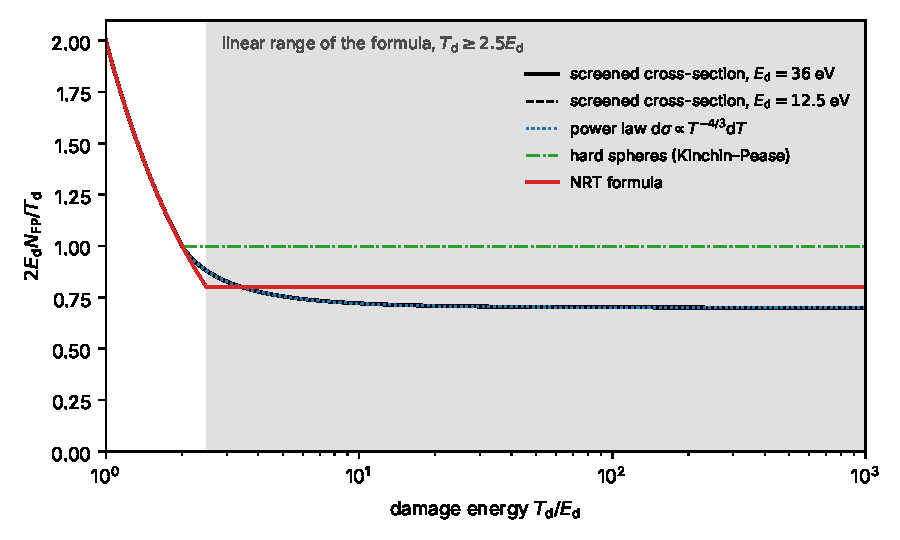
\includegraphics[width=\linewidth]{figures/ch19/limit19_4a.pdf}
\captionof{figure}{Displaced atoms per Kinchin--Pease unit, $2E_{\mathrm{d}}N_{\mathrm{FP}}/T_{\mathrm{d}}$, against $T_{\mathrm{d}}/E_{\mathrm{d}}$, from the counting equation \cref{eq:19.4-count} with the Kinchin--Pease rules, no binding energy and no electronic loss. Solid and dashed black: the Thomas--Fermi cross-section of \cref{sec:19.3} (impulse deflection, continued below $x_L = 2\times10^{-3}$ as $x_L^{1/3}$) for silicon with $E_{\mathrm{d}} = 36$ and \SI{12.5}{eV}; dotted: the power law $T^{-4/3}$; dash-dotted: hard spheres, which reproduce \cref{eq:19.4-KP} exactly. Red: the formula. Gray: $T_{\mathrm{d}} \ge 2.5E_{\mathrm{d}}$, the formula's linear range.}\label{fig:19-limit-nrt}
\par}
\smallskip
In its linear range the formula lies 11 to \SI{14}{\percent} above the screened count for $T_{\mathrm{d}} \ge 10E_{\mathrm{d}}$ and \SI{20}{\percent} below the hard-sphere count; below $2.5E_{\mathrm{d}}$ the count is set by the direction dependence of the threshold and by recombination, which no counting rule contains.
\end{limitbox}

The factor in front of the count is therefore a property of the cross-section and of the rules, not a constant of the crystal: 1 for hard spheres, 0.8 in the formula, 0.70 for the screened cross-section that \cref{sec:19.3} uses for Lindhard quenching. The rules leave out binding and recombination. A binding energy paid by every displaced atom lowers the count. Recombination inside a dense cascade lowers the number of defects that survive; in metals the surviving number from molecular dynamics is a third to a quarter of the formula's count~\cite{nordlund2018improving}, while silicon and germanium recombine much less~\cite[Sect.~II\,B]{sassi2022energy}.

The defect energy loss follows by multiplying the count by the surviving fraction and by the energy per pair. Writing $E_{\mathrm{FP}}$ for the mean stored energy of a surviving displacement,
\begin{equation}
  \frac{\langle E_{\mathrm{st}}\rangle}{E_R} = \frac{\xi_{\mathrm{d}}}{2}\,\frac{T_{\mathrm{d}}}{E_R}\,\frac{p_{\mathrm{surv}}E_{\mathrm{FP}}}{E_{\mathrm{d}}} \qquad (T_{\mathrm{d}} \gg E_{\mathrm{d}}) .
  \label{eq:19.4-loss}
\end{equation}
The stored fraction depends on the recoil energy only through the damage fraction $T_{\mathrm{d}}/E_R = 1 - y_L$, which falls from 0.70 at \SI{10}{keV} to 0.49 at \SI{100}{keV} for silicon in Lindhard's model, \cref{eq:16.6-lindhard}. At fixed $p_{\mathrm{surv}}E_{\mathrm{FP}}$ it decreases as $1/E_{\mathrm{d}}$: a higher threshold means fewer displacements, each storing the same energy. A measured stored fraction fixes only the combination $\xi_{\mathrm{d}}p_{\mathrm{surv}}E_{\mathrm{FP}}/E_{\mathrm{d}}$.

\begin{workedexample}{Energy stored by a 300 eV silicon recoil}\label{we:19-fp300}
A silicon recoil of \SI{300}{eV} needs $\mchi \ge \SI{0.770}{GeV}$ by \cref{eq:1.3-ERmax}, with $M_\kappa = \SI{26.16}{GeV}$ (natural isotope mixture, as in \cref{sec:19.1}) and $v_{\mathrm{max}} = \num{2.650e-3}$. Its measured ionization yield, interpolated linearly in $\ln Y_q$ against $\ln E_R$ between 0.108 at \SI{0.22}{keV} and 0.136 at \SI{0.46}{keV}~\cite[Table~II]{albakry2023first}, is $Y_q = 0.119$. The electronic share is at most $Y_qE_R = \SI{36}{eV}$, since the near-gap excitations of a slow ion each cost less than $\varepsilon_{\mathrm{eh}}$ per pair (\cref{sec:19.2}), so $T_{\mathrm{d}} \ge \SI{264}{eV}$; we take this value.

With the average Frenkel-pair threshold $E_{\mathrm{d}} = \SI{36}{eV}$, $T_{\mathrm{d}}/E_{\mathrm{d}} = 7.34$. The hard-sphere count \cref{eq:19.4-KP} gives 3.67 displacements, the formula of \cref{lim:19.4a} 2.94, and the screened count of \cref{eq:19.4-count} 2.69. If every displacement survives as a close pair of 6.8 to \SI{7.5}{eV}, the recoil stores 18.3 to \SI{20.1}{eV}, 6.1 to \SI{6.7}{\percent} of its energy; as separated pairs of 8.1 to \SI{9.7}{eV}, 22 to \SI{26}{eV}, or 7.3 to \SI{8.7}{\percent}. With the threshold for a defect of either kind, \SI{24}{eV}, the screened count is 3.95, and bond defects alone would store 10 to \SI{12}{eV}.

These fractions are comparable to the deficits measured at 10 to \SI{100}{keV}, and a calorimeter calibrated with electron recoils would read this recoil about \SI{20}{eV} low.
\end{workedexample}
